\documentclass{amsart}

\usepackage[utf8]{inputenc}
\usepackage{amsthm,mathtools,tikz}
\usetikzlibrary{patterns,matrix}
\usepackage[protrusion=true,expansion=true]{microtype}
\usepackage{hyperref}

\usepackage[natbib=true,style=numeric,maxnames=10]{biblatex}
\usepackage[babel]{csquotes}
\bibliography{paper-generic-freeness.bib}

\title[Grothendieck's generic freeness lemma]{An elementary and constructive
proof of Grothendieck's generic freeness lemma}
\author{Ingo Blechschmidt}

\theoremstyle{definition}
\newtheorem{defn}{Definition}[]
\newtheorem{ex}[defn]{Example}

\theoremstyle{plain}
\newtheorem{prop}[defn]{Proposition}
\newtheorem{cor}[defn]{Corollary}
\newtheorem{lemma}[defn]{Lemma}
\newtheorem{thm}[defn]{Theorem}
\newtheorem{scholium}[defn]{Scholium}

\theoremstyle{remark}
\newtheorem{rem}[defn]{Remark}
\newtheorem{question}[defn]{Question}
\newtheorem{speculation}[defn]{Speculation}
\newtheorem{caveat}[defn]{Caveat}
\newtheorem{conjecture}[defn]{Conjecture}

\newcommand{\XXX}[1]{\textbf{XXX: #1}}
\newcommand{\aaa}{\mathfrak{a}}
\newcommand{\bbb}{\mathfrak{b}}
\newcommand{\defeq}{\vcentcolon=}
\DeclareMathOperator{\Spec}{Spec}

\newcommand{\stacksproject}[1]{\cite[{\href{https://stacks.math.columbia.edu/tag/#1}{Tag~#1}}]{stacks-project}}

\begin{document}

\begin{abstract}
  We present a new and direct proof of Grothendieck's generic freeness
  lemma in its general form. Unlike the previously published proofs, it doesn't
  proceed in a series of reduction steps and is fully constructive, not
  involving the axiom of choice or even the law of excluded middle. It was
  found by unwinding the result of a general topos-theoretic technique.
\end{abstract}

\maketitle

\noindent
We prove Grothendieck's generic freeness lemma for rings and modules in the
following form.

\begin{thm}\label{thm:algebraic}Let~$A$ be a reduced ring. Let~$B$ be
an~$A$-algebra of finite type. Let~$M$ be a finitely generated~$B$-module.
If~$f = 0$ is the only element of~$A$ such that
\begin{enumerate}
\item the~$A[f^{-1}]$-modules $B[f^{-1}]$ and $M[f^{-1}]$ are free,
\item the~$A[f^{-1}]$-algebra~$B[f^{-1}]$ is of finite presentation, and
\item the~$B[f^{-1}]$-module~$M[f^{-1}]$ is finitely presented,
\end{enumerate}
then~$1 = 0$ in~$A$.
\end{thm}

Previously known proofs either only cover the case where~$A$ is a Noetherian
integral domain, where one can argue by \emph{dévissage} (see for
instance~\cite[Lemme~6.9.2]{ega-4-2},
\cite[Thm.~24.1]{matsumura:commutative-ring-theory}, or
\cite[Thm.~14.4]{eisenbud:commutative-algebra}), or proceed in a series of
intermediate steps, reducing to that case (see for
instance~\cite{staats:generic-freeness} or~\stacksproject{051Q}); but in fact,
a direct proof is possible and shorter.

Grothendieck's generic freeness lemma is often presented in contrapositive form
or in the following geometric variant:

\begin{thm}\label{thm:geometric}Let~$A$ be a reduced ring. Let~$B$ be
an~$A$-algebra of finite type. Let~$M$ be a finitely generated~$B$-module. Then
the space~$\Spec(A)$ contains a dense open~$U$ such that over~$U$,
\begin{enumerate}
\item[(a)] $B^\sim$ and~$M^\sim$ are free as sheaves of~$A^\sim$-modules,
\item[(b)] $B^\sim$ is of finite presentation as a sheaf of~$A^\sim$-algebras, and
\item[(c)] $M^\sim$ is finitely presented as a sheaf of~$B^\sim$-modules.
\end{enumerate}
\end{thm}

Theorem~\ref{thm:geometric} immediately follows from
Theorem~\ref{thm:algebraic} by defining~$U$ as the union of all the basic
opens~$D(f)$ such that~(1),~(2), and~(3) hold. It's clear that~(a),~(b),
and~(c) hold over~$U$, and~$U$ is dense for if~$V$ is an arbitrary open
such that~$U \cap V = \emptyset$, the open~$V$ is itself empty: Let~$h \in A$
such that~$D(h) \subseteq V$. The hypothesis implies the assumptions of
Theorem~\ref{thm:algebraic} for the datum~$(A[h^{-1}], B[h^{-1}], M[h^{-1}])$.
Thus~$1 = 0 \in A[h^{-1}]$, so~$h$ is nilpotent and~$D(h) = \emptyset$.

The new proof was found using a general topos-theoretical technique which we
believe to be useful in other situations as well. This technique allows to view
reduced rings and their modules from a different point of view, one from which
reduced rings look like fields. Since Grothendieck's generic freeness
is trivial for fields, this technique yields a trivial proof for reduced rings.
The proof presented here was obtained by unwinding the topos-theoretic proof,
yielding a self-contained argument without any references to topos theory.
We refer readers who want to learn about this technique to a companion 
paper~\cite{blechschmidt:wlog}.

\textbf{Acknowledgments.} The proof presented here was prompted by
user~HeinrichD on MathOverflow~\cite{mo:kernel} and greatly
benefited from discussions with Martin Brandenburg, who needed the constructive
version in a paper of his~\cite{brandenburg:schur}. I'm grateful to Marc
Nieper-Wißkirchen for carefully guiding my PhD thesis, where \XXX{...}


\section{The proof of the general case}

\begin{lemma}\label{lemma:basis}
Let~$A$ be a ring. Let~$M$ be an~$A$-module with generating
family~$(x_i)_{i \in I}$ where~$I$ is a totally ordered set. Assume that the
only element~$g \in A$ such that one of the~$x_i$ is an~$A[g^{-1}]$-linear
combination in~$M[g^{-1}]$ of other generators with smaller index is~$g = 0$.
Then~$M$ is free with~$(x_i)_{i \in I}$ as a basis.
\end{lemma}

\begin{proof}Let~$\sum_i a_i x_i = 0$. Starting with the greatest
index~$i$ which appears in that sum, we see that in~$M[a_i^{-1}]$, the
element~$x_i$ is an~$A[g^{-1}]$-linear combination of other generators with
smaller index. Thus~$a_i = 0$ by assumption.\end{proof}

\begin{proof}[Proof of Theorem~\ref{thm:algebraic}]
Let~$B$ be generated by~$(x_1,\ldots,x_n)$ as an~$A$-algebra and
let~$M$ be generated by~$(v_1,\ldots,v_m)$ as a~$B$-module. We endow the sets
\begin{align*}
  I &\defeq \{ (i_1,\ldots,i_n) \,|\, i_1,\ldots,i_n \in \{ 0,1,\ldots \} \}
  \quad\text{and} \\
  J &\defeq \{ (\ell, i_1,\ldots,i_n) \,|\, \ell \in \{ 1,\ldots,m \}, i_1,\ldots,i_n \in \{ 0,1,\ldots \} \}
\end{align*}
with the lexicographic order. The family~$(w_j)_{j \in J} \defeq (x_1^{i_1}
\cdots x_n^{i_n} v_\ell)_{(\ell,i_1,\ldots,i_n) \in J}$ generates~$M$ as
an~$A$-module, and we'll call a subfamily~$(w_j)_{j \in J' \subseteq J}$
\emph{good} if and only if for all~$j \in J$, the vector~$w_j$ is a linear
combination of the vectors~$(w_{j'})_{j' \in J, j' \preceq j}$,
and if~$(\ell,i_1,\ldots,i_n) \not\in J'$ implies~$(\ell,k_1,\ldots,k_n) \not\in
I'$ for all~$k_1 \geq i_1, \ldots, k_n \geq i_n$. Figure~\ref{fig:good} shows
how a good generating family can look like.

\begin{figure}[b]
  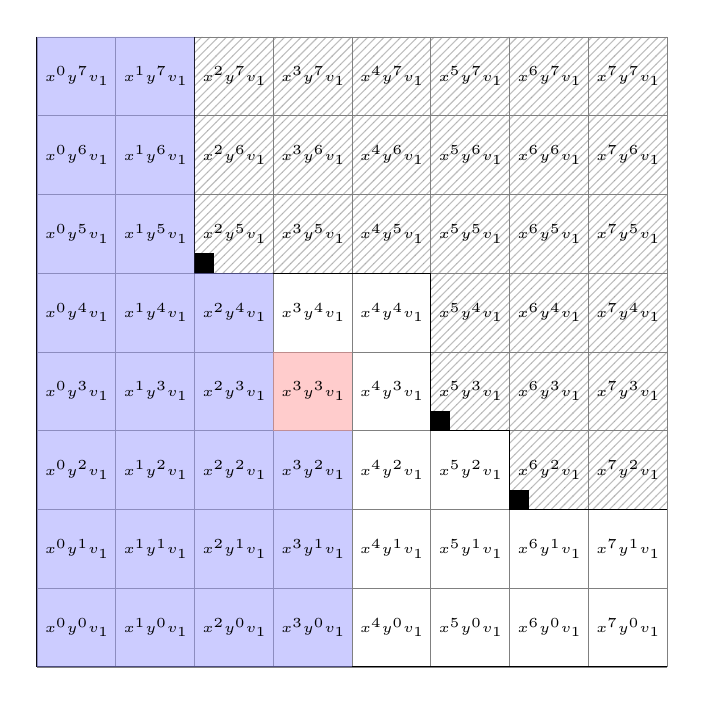
\begin{tikzpicture}[scale=1.0]
    \draw[step=1cm,gray,very thin] (0,0) grid (8,8);

    \draw
      (0,8) -- (0,0) -- (8,0);

    \fill[pattern=north east lines,pattern color=gray,opacity=0.5]
      (2,8) -- (2,5) -- (5,5) -- (5,3) -- (6,3) -- (6,2) -- (8,2) -- (8,8);
    \draw
      (2,8) -- (2,5) -- (5,5) -- (5,3) -- (6,3) -- (6,2) -- (8,2);

    \fill[fill=black] (2,5.25) -- (2,5) -- (2.25,5) -- (2.25,5.25);
    \fill[fill=black] (5,3.25) -- (5,3) -- (5.25,3) -- (5.25,3.25);
    \fill[fill=black] (6,2.25) -- (6,2) -- (6.25,2) -- (6.25,2.25);

    \fill[fill=blue!40!white,opacity=0.5]
      (0,8) -- (0,0) -- (4,0) -- (4,3) -- (3,3) -- (3,5) -- (2,5) -- (2,8);

    \fill[fill=red!40!white,opacity=0.5]
      (3,3) -- (4,3) -- (4,4) -- (3,4);

    % !perl -we 'for my $y (reverse 0..7) { for my $x (0..7) { print % "\$x^$x\Ey^$y\$ & " } print "\\\\ \n" }'
    \begin{scope}[yshift=4cm, xshift=4cm]
      \matrix[matrix of nodes,nodes={inner sep=0pt,text width=1.0cm,align=center,minimum height=1.0cm}]{
        \tiny $x^0y^7v_1$ & \tiny $x^1y^7v_1$ & \tiny $x^2y^7v_1$ & \tiny $x^3y^7v_1$ & \tiny $x^4y^7v_1$ & \tiny $x^5y^7v_1$ & \tiny $x^6y^7v_1$ & \tiny $x^7y^7v_1$ & \\
        \tiny $x^0y^6v_1$ & \tiny $x^1y^6v_1$ & \tiny $x^2y^6v_1$ & \tiny $x^3y^6v_1$ & \tiny $x^4y^6v_1$ & \tiny $x^5y^6v_1$ & \tiny $x^6y^6v_1$ & \tiny $x^7y^6v_1$ & \\
        \tiny $x^0y^5v_1$ & \tiny $x^1y^5v_1$ & \tiny $x^2y^5v_1$ & \tiny $x^3y^5v_1$ & \tiny $x^4y^5v_1$ & \tiny $x^5y^5v_1$ & \tiny $x^6y^5v_1$ & \tiny $x^7y^5v_1$ & \\
        \tiny $x^0y^4v_1$ & \tiny $x^1y^4v_1$ & \tiny $x^2y^4v_1$ & \tiny $x^3y^4v_1$ & \tiny $x^4y^4v_1$ & \tiny $x^5y^4v_1$ & \tiny $x^6y^4v_1$ & \tiny $x^7y^4v_1$ & \\
        \tiny $x^0y^3v_1$ & \tiny $x^1y^3v_1$ & \tiny $x^2y^3v_1$ & \tiny $x^3y^3v_1$ & \tiny $x^4y^3v_1$ & \tiny $x^5y^3v_1$ & \tiny $x^6y^3v_1$ & \tiny $x^7y^3v_1$ & \\
        \tiny $x^0y^2v_1$ & \tiny $x^1y^2v_1$ & \tiny $x^2y^2v_1$ & \tiny $x^3y^2v_1$ & \tiny $x^4y^2v_1$ & \tiny $x^5y^2v_1$ & \tiny $x^6y^2v_1$ & \tiny $x^7y^2v_1$ & \\
        \tiny $x^0y^1v_1$ & \tiny $x^1y^1v_1$ & \tiny $x^2y^1v_1$ & \tiny $x^3y^1v_1$ & \tiny $x^4y^1v_1$ & \tiny $x^5y^1v_1$ & \tiny $x^6y^1v_1$ & \tiny $x^7y^1v_1$ & \\
        \tiny $x^0y^0v_1$ & \tiny $x^1y^0v_1$ & \tiny $x^2y^0v_1$ & \tiny $x^3y^0v_1$ & \tiny $x^4y^0v_1$ & \tiny $x^5y^0v_1$ & \tiny $x^6y^0v_1$ & \tiny $x^7y^0v_1$ & \\
      };
    \end{scope}
  \end{tikzpicture}
  \caption{\label{fig:good}A graphical depiction of a good generating family in
  the special case~$n = 2, m = 1$. The hatched cells indicate vectors which
  have already been removed from the family. The small black squares indicate
  \emph{corners}. If the vector in the red cell will be found to be expressible
  as a linear combination of vectors with smaller index (blue cells), it will
  be removed, along with the vectors in all cells to the top and to the right
  of the red cell.}
\end{figure}

Similarly, we define when a subfamily of the canonical generating
family~$(x_1^{i_1} \cdots x_n^{i_n})_{(i_1,\ldots,i_n) \in I}$ of~$B$ is good
(which is just the special case~$m = 1$). We then proceed by induction on the
shapes of a given good generating family~$(w_j)_{j \in J'}$ for~$M$ and a given
good generating family~$(s_i)_{i \in I'}$ for~$B$, starting with the canonical
ones.

We show that~$(w_j)_{j \in J'}$ is a basis of~$M$ by verifying the assumptions
of Lemma~\ref{lemma:basis}. Thus let~$g \in A$ be given such that one of
the~$w_j$ is an $A[g^{-1}]$-linear combination of generators with smaller index
in~$M[g^{-1}]$. Removing~$w_j = x_1^{i_1} \cdots x_n^{i_n} v_\ell$ and also all
vectors~$x_1^{k_1} \cdots x_n^{k_n} v_\ell$ where~$k_1 \geq i_1, \ldots,
k_n \geq i_n$, we obtain a subfamily which is still good for
the~$A[g^{-1}]$-module~$M[g^{-1}]$. By induction, applied
to~$A[g^{-1}]$ and its module~$M[g^{-1}]$, it therefore follows that $A[g^{-1}] = 0$.
This implies that $g = 0$ since~$A$ is reduced.

Similarly, we show that the given good generating family~$(s_i)_{i \in I'}$ is
a basis. Thus~$M$ and~$B$ are free over~$A$. We fix for any corner~$j =
(\ell,i_1,\ldots,i_n) \in J$, as indicated in Figure~\ref{fig:good},
a way of expressing~$x^{i_1} \cdots x^{i_n} v_\ell = \sum_{(p,k_1,\ldots,k_n)}
a_{j; p,k_1,\ldots,k_n} x^{k_1} \cdots x^{k_n} v_p$ as a linear combination of
generators with strictly smaller index. Then~$M$ is isomorphic to
the~$B$-module
\[ B\langle V_1,\ldots, V_m\rangle/
  (x^{i_1} \cdots x^{i_n} V_\ell - \textstyle\sum_{(p,k_1,\ldots,k_n)}
  a_{j; p,k_1,\ldots,k_n} x_{k_1} \cdots x_{k_n} V_p)_j,
\]
where the index~$j$ ranges over all corners of~$J$, and is therefore finitely
presented. In a similar vain, a quotient algebra of~$A[X_1,\ldots,X_n]$, where
we mod out a suitable ideal with as many generators as corners of~$I$, is
isomorphic to~$B$.

We finish by using the assumption for~$f = 1$.
\end{proof}


\section{The proof of the finitely-generated case}

The following proposition is just an instance of Grothendieck's generic
freeness lemma. We present it here because it admits an easier proof.

\begin{prop}Let~$A$ be a reduced ring. Let~$M$ be a finitely
generated~$A$-module. If~$f = 0$ is the only element of~$A$ such
that~$M[f^{-1}]$ is a finite free~$A[f^{-1}]$-module, then~$1 = 0$ in~$A$.
\end{prop}

\begin{proof}We proceed by induction on the length of a given generating family
of~$M$. Let~$M$ be generated by~$(v_1,\ldots,v_m)$.

We show that the family~$(v_1,\ldots,v_m)$ is linearly independent. Let~$\sum_i
a_i v_i = 0$. Over~$A[a_i^{-1}]$, the vector~$v_i \in M[a_i^{-1}]$ is a linear
combination of the other generators. Thus~$M[a_i^{-1}]$ can be generated as
an~$A[a_i^{-1}]$-module by fewer than~$m$ generators. The induction hypothesis,
applied to this module, yields that~$1 = 0$ in~$A[a_i^{-1}]$. Since~$A$ is
reduced, this amounts to~$a_i = 0$.

We finish by using the assumption for~$f = 1$.
\end{proof}

\printbibliography


\end{document}

Recall that a module is Noetherian if and only if all of its submodules are
finitely generated. We call a module~$M$ over an~$A$-algebra~$B$ \emph{weakly
Noetherian} (over~$A$) if and only if, for all~$B$-submodules~$U \subseteq M$
and all~$f \in A$ the condition
\begin{multline*}
  \text{for all~$g \in A$, if $U[(fg)^{-1}]$ is finitely generated as
an~$B[(fg)^{-1}]$-module,} \\
  \text{then~$fg$ is nilpotent in~$A$} \end{multline*}
implies that~$f$ is nilpotent. Geometrically, this expresses that all
quasicoherent sheaves of submodules of~$M^\sim$ are, over a dense open
of~$\Spec(A)$, of finite type over~$B^\sim$. An~$A$-algebra~$B$
is \emph{weakly Noetherian} if and only if it is weakly Noetherian as a module
over itself.

This notion is interesting for the following reason.

\begin{lemma}\label{lemma:self-noetherian}
Let~$A$ be a reduced ring. Then~$A$, regarded as an algebra over itself, is
weakly Noetherian.\end{lemma}

\begin{proof}Let~$\aaa \subseteq A$ be an ideal. Let~$f \in A$ such that, for
any~$g \in A$, if~$\aaa[(fg)^{-1}]$ is finitely generated, then~$fg = 0$.
We verify that~$f = 0$.

We first show that~$\aaa[f^{-1}] = (0)$. Let~$g \in \aaa$. Then~$\aaa[(fg)^{-1}] =
(1)$ is finitely generated. Thus~$fg = 0$, hence~$g = 0$ in~$A[f^{-1}]$.

Since~$\aaa[f^{-1}]$ is finitely generated, we finish by using the
assumption for~$g = 1$.
\end{proof}

The weak Noetherian condition enjoys the same basic stability properties as the
usual Noetherian condition:

\begin{lemma}\label{lemma:noetherian-stability}
Let~$A$ be a ring. Let~$B$ be an~$A$-algebra.
\begin{enumerate}
\item If~$B$ is weakly Noetherian, then so is~$B[X]$.
\item Let~$0 \to M' \to M \to M'' \to 0$ be a short exact sequence
of~$B$-modules. Then~$M$ is weakly Noetherian if and only if~$M'$ and~$M''$
are.
\end{enumerate}
\end{lemma}

We can use these observations to finish the proof of Grothendieck's generic
freeness lemma.

\begin{prop}Let~$A$ be a reduced ring. Let~$B$ be an~$A$-algebra of finite type.
If~$f = 0$ is the only element of~$A$ such that~$B[f^{-1}]$ is of finite
presentation as an~$A[f^{-1}]$-algebra, then~$1 = 0$ in~$A$.
\end{prop}

\begin{proof}We write~$B = A[X_1,\ldots,X_n]/\aaa$. By Lemma~\ref{lemma:self-noetherian} and
Lemma~\ref{lemma:noetherian-stability}, the~$A$-algebra~$A[X_1,\ldots,X_n]$ is
weakly Noetherian. We can therefore conclude if we can show, for any~$g \in A$,
that if the ideal~$\aaa[g^{-1}]$ is finitely generated, then~$g = 0$. This
follows immediately from the assumption (for~$f = g$).
\end{proof}

\begin{prop}Let~$A$ be a reduced ring. Let~$B$ be an~$A$-algebra of finite type.
Let~$M$ be a finitely generated~$B$-module. If~$f = 0$ is the only element
of~$A$ such that~$M[f^{-1}]$ is finitely presented as an~$B[f^{-1}]$-module,
then~$1 = 0$ in~$A$.
\end{prop}

\begin{proof}We write~$M = B^n/U$ for an~$B$-submodule~$U$. By Lemma~\ref{lemma:self-noetherian} and
Lemma~\ref{lemma:noetherian-stability}, the~$B$-module~$B^n$ is weakly
Noetherian. We can therefore conclude if we can show, for any~$g \in A$, that if
the submodule~$U[g^{-1}]$ is finitely generated, then~$g = 0$. This follows
immediately from the assumption (for~$f = g$).
\end{proof}

\end{document}
